% !TeX root = booklet-01.tex
\section{از شماتیک تا مقطع و نمای بالا}
\label{sec:layout-views}
\subsection{سه نمایش از یک مدار}
شماتیک می‌گوید کدام پایانه‌ها به هم وصل‌اند؛ فاصله و اندازه خطوط آن عموماً معنای
ساخت ندارد. \lr{Layout} نمای بالای هندسه لایه‌هاست و محل و ابعاد اجزا را مشخص می‌کند.
\lr{Cross-section} برش عمودی از یک مسیر مشخص روی همان \lr{Layout} است؛
فقط اجزایی را نشان می‌دهد که صفحه برش از آن‌ها می‌گذرد
\cite[بخش \secnum{۱.۵} و شکل‌های \secnum{۱.۳۴} و \secnum{۱.۳۵}]{weste}.
پس ممکن است دو \lr{Gate} در شماتیک متصل باشند، ولی سیم مشترک آن‌ها در مقطع خاص دیده نشود.
برای فهم مدار باید اتصال‌های خارج از صفحه برش را نیز از نمای بالا یا برچسب‌ها خواند.

\lr{Layer} در نقشه، یک رده هندسه یا یک مرحله تعریف فرایند است.
هر رنگ لزوماً یک ورقه رسانای مجزا نیست؛ مثلاً \lr{n-well} ناحیه‌ای در خود
نیمه‌هادی و \lr{Contact} محل بازشدن عایق برای اتصال است.
دو مستطیل که از بالا هم‌پوشانی دارند، ممکن است در ارتفاع‌های متفاوت و عایق‌شده باشند.
این نکته در خواندن تقاطع \lr{Metal} و \lr{Poly} ضروری است.

\subsection{مقطع \lr{CMOS Inverter} و اتصال پایانه‌های آن}
در مثال کتاب، بستر \lr{p-substrate} است. \lr{nMOS} در همان بستر و
\lr{pMOS} در ناحیه \lr{n-well} ساخته می‌شود.
هر \lr{nMOS} دو ناحیه \(n^+\) و هر \lr{pMOS} دو ناحیه \(p^+\)
برای \lr{Source} و \lr{Drain} دارد.
علامت \(+\) شدت زیاد \lr{Doping} را نشان می‌دهد، نه بار مثبت ناحیه
\cite[بخش \secnum{۱.۵.۱}]{weste}.

در \lr{Inverter}، \lr{Source} ترانزیستور پایین به زمین، \lr{Source}
ترانزیستور بالا به تغذیه، دو \lr{Drain} به خروجی \(Y\) و دو \lr{Gate}
به ورودی \(A\) متصل‌اند. بدنه \lr{nMOS} باید مرجع پایین و بدنه \lr{pMOS}
مرجع بالا را بگیرد. شکل \ref{fig:layout-crosssection} این ساختار را به‌شکل ساده نشان می‌دهد.

\begin{figure}[ht]
\centering
\begin{latin}
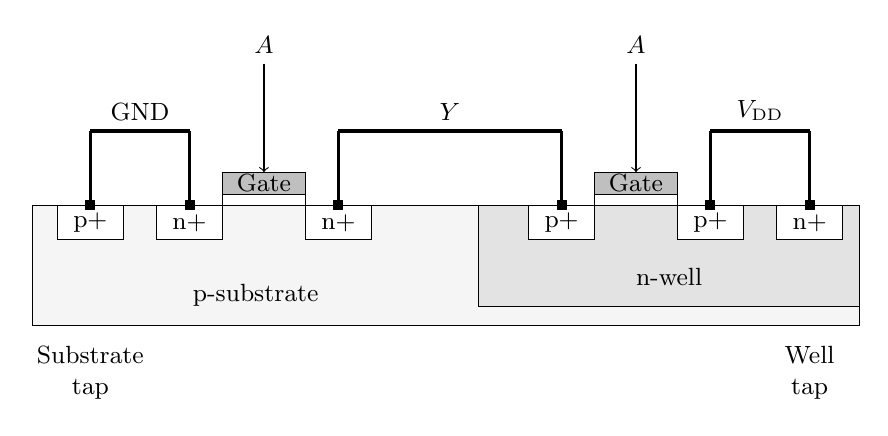
\begin{tikzpicture}[x=1.05cm,y=0.95cm,font=\small]
\draw[fill=gray!8] (0,0) rectangle (10,1.6);
\draw[fill=gray!22] (5.4,0.25) rectangle (10,1.6);
\node at (2.7,0.4) {p-substrate};\node at (7.7,0.65) {n-well};
\foreach \a/\b/\lab in {0.3/1.1/p+,1.5/2.3/n+,3.3/4.1/n+,6/6.8/p+,7.8/8.6/p+,9/9.8/n+} {
\draw[fill=white] (\a,1.15) rectangle (\b,1.6);
\node at ({(\a+\b)/2},1.37) {\lab};}
\foreach \a/\b in {2.3/3.3,6.8/7.8} {
\draw[fill=white] (\a,1.6) rectangle (\b,1.75);
\draw[fill=gray!50] (\a,1.75) rectangle (\b,2.05);}
\node at (2.8,1.9) {Gate};\node at (7.3,1.9) {Gate};
\foreach \x in {0.7,1.9,3.7,6.4,8.2,9.4} {
\draw[very thick] (\x,1.6)--(\x,2.6);
\fill (\x-0.06,1.55) rectangle (\x+0.06,1.68);}
\draw[very thick] (0.7,2.6)--(1.9,2.6) node[midway,above] {GND};
\draw[very thick] (3.7,2.6)--(6.4,2.6) node[midway,above] {$Y$};
\draw[very thick] (8.2,2.6)--(9.4,2.6) node[midway,above] {$V_{\mathrm{DD}}$};
\draw[->] (2.8,3.5) node[above] {$A$}--(2.8,2.05);
\draw[->] (7.3,3.5) node[above] {$A$}--(7.3,2.05);
\node[below,align=center] at (0.7,-0.15) {Substrate\\tap};
\node[below,align=center] at (9.4,-0.15) {Well\\tap};
\end{tikzpicture}
\end{latin}
\caption{طرح مفهومی مقطع \lr{Inverter} بر پایه شکل \secnum{۱.۳۴} کتاب \cite{weste}.
ابعاد و ارتفاع‌ها واقعی نیستند؛ خط‌های ضخیم اتصال رسانشی و مربع‌های کوچک محل تماس‌اند.
فضای بالای بستر، به‌جز محل تماس و رساناها، عایق فرض شده است.
دو \lr{Gate} با برچسب \(A\) در خارج از این برش به هم وصل می‌شوند.}
\label{fig:layout-crosssection}
\end{figure}

\subsection{چرا \lr{Tap} لازم است؟}
\lr{Substrate Tap} یک ناحیه \(p^+\) در بستر \lr{p} و \lr{Well Tap}
یک ناحیه \(n^+\) داخل چاه \lr{n} است. تماس فلزی با این ناحیه‌های پرناخالصی،
اتصال کم‌مقاومت به بدنه را فراهم می‌کند.
تماس با نیمه‌هادی کم‌ناخالصی می‌تواند رفتار \lr{Schottky} و یکسوساز داشته باشد؛
\lr{Doping} زیاد برای تماس \lr{Ohmic} مناسب است
\cite[صفحه چاپی ۲۰]{weste}.

اتصال بستر به زمین و چاه به تغذیه، در محدوده معمول ولتاژهای مدار، از
بایاس مستقیم ناخواسته پیوندهای بدنه با \lr{Source/Drain} جلوگیری می‌کند.
\textbf{تماس \lr{Source} جای \lr{Tap} بدنه را نمی‌گیرد.}
در \lr{nMOS}، ناحیه \(n^+\) مربوط به \lr{Source} و ناحیه \(p^+\)
مربوط به بدنه، دو ناحیه متفاوت‌اند؛ حتی اگر هر دو با فلز به زمین متصل شوند.
به همین ترتیب \lr{pMOS} برای بدنه \lr{n-well} به تماس \(n^+\) نیاز دارد.

\subsection{نقش عایق نازک، عایق میدان و تماس}
\lr{Gate Oxide} لایه نازک میان \lr{Gate} و کانال است؛ میدان را منتقل
می‌کند، ولی در مدل ایدئال مسیر رسانشی مستقیم نیست.
\lr{Field Oxide} و عایق‌های بین لایه‌ها، ناحیه‌ها و فلز را از مسیرهای
ناخواسته جدا می‌کنند. سوراخ \lr{Contact} فقط در محل مجاز، اتصال فلز به
\lr{Diffusion} یا \lr{Poly} را برقرار می‌کند.
اتصال میان دو لایه فلزی را معمولاً \lr{Via} می‌نامیم.
پس روی هم افتادن \lr{Metal1} و \lr{Poly} بدون \lr{Contact}، آن‌ها را اتصال کوتاه نمی‌کند.

در مدل ساده این فصل، \lr{Poly} روی ناحیه فعال از عایق نازک جدا می‌شود و
ترانزیستور را می‌سازد. این تقاطع نیز اتصال کوتاه \lr{Gate} به کانال نیست.
تفاوت میان «تماس»، «تقاطع ترانزیستوری» و «عبور عایق‌شده» را در همه شکل‌ها حفظ می‌کنیم.

\section{مراحل آموزشی \lr{Fabrication}}
\label{sec:layout-fabrication}
\subsection{ماسک چیست و چرا شش ماسک کافیِ واقعی نیست؟}
\lr{Mask} الگوی هندسی انتخاب ناحیه‌ها در یک مرحله فرایند است.
کتاب برای توضیح \lr{Inverter} از مجموعه فرضی شش ماسک شامل
\lr{n-well}، \lr{Polysilicon}، \lr{n-diffusion}، \lr{p-diffusion}،
\lr{Contact} و \lr{Metal} استفاده می‌کند
\cite[بخش \secnum{۱.۵.۲} و شکل \secnum{۱.۳۵}]{weste}.
این شش نام، مراحل کامل یک فرایند صنعتی نیستند.
به‌ویژه هندسه‌های نهایی \lr{Layout} لزوماً با ماسک‌های واقعیِ بیشتر و اصلاح‌شده،
رابطه یک‌به‌یک ندارند.

\lr{Photolithography} با استفاده از نور و \lr{Photoresist}، الگوی ماسک
را روی لایه‌ای حساس منتقل می‌کند. \lr{Etching} ماده را از ناحیه‌های بازشده
برمی‌دارد. \lr{Deposition} ماده اضافه می‌کند و \lr{Oxidation} لایه اکسید را
با واکنش روی سطح ایجاد می‌کند. \lr{Doping} نوع و غلظت حامل‌ها را در ناحیه انتخاب‌شده تغییر می‌دهد.
این عمل‌ها نقش یکسان ندارند؛ برداشتن \lr{Photoresist} به معنی حذف چاه یا رسانای زیر آن نیست.

\subsection{ساخت \lr{n-well}: الگوگذاری را مرحله‌به‌مرحله دنبال کنیم}
شکل \secnum{۱.۳۶} کتاب، ساخت چاه را در چند مقطع نشان می‌دهد. ترتیب آموزشی آن چنین است
\cite[صفحات چاپی ۲۱ تا ۲۳]{weste}:
\begin{enumerate}
\item از ویفر \lr{p-type} آغاز می‌کنیم. کل ویفر، یک تراشه منفرد نیست؛
ناحیه‌های چندین تراشه روی آن پردازش می‌شوند.
\item یک اکسید محافظ روی سطح تشکیل می‌شود. در مثال کتاب، رشد حرارتی اکسید
با واکنش \lr{Si} و اکسیژن انجام می‌شود؛ این لایه در این مرحله سد انتخاب ناحیه است.
\item سطح با \lr{Photoresist} پوشانده و از پشت ماسک چاه نوردهی می‌شود.
کتاب نوعی رفتار مثبت را توصیف می‌کند: بخش نورخورده در مرحله \lr{Develop} حذف می‌شود.
این قرارداد را نباید بی‌قید به همه انواع \lr{Resist} تعمیم داد.
\item در ناحیه باز \lr{Resist}، اکسید \lr{Etch} می‌شود؛ اکسید زیر بخش
محافظت‌شده باقی می‌ماند. پس اکنون سوراخی در سد اکسیدی داریم.
\item \lr{Resist} باقی‌مانده پاک می‌شود؛ ماسک اکسیدی هنوز روی ویفر وجود دارد.
این تمایز لازم است، چون مرحله ورود ناخالصی باید همچنان انتخابی باشد.
\item ناخالصی مناسب \lr{n-type} در ناحیه باز وارد می‌شود تا نوع آن بخش
از بستر تغییر کند و چاه تشکیل شود. انتشار جانبی می‌تواند مرز نهایی را
با لبه هندسی سوراخ یکسان نگه ندارد.
\item اکسید محافظ باقی‌مانده پاک می‌شود؛ چاه که داخل نیمه‌هادی تشکیل شده،
با برداشتن اکسید از بین نمی‌رود.
\end{enumerate}

شکل \ref{fig:layout-well-stages} سه مقطع از همین مسیر را کنار هم می‌گذارد.
در مقطع میانی، \lr{Resist} برداشته شده ولی سد اکسیدی باقی است؛
با مقطع نهایی که اکسید محافظ حذف شده تفاوت دارد.
\begin{figure}[ht]
\centering
\begin{latin}
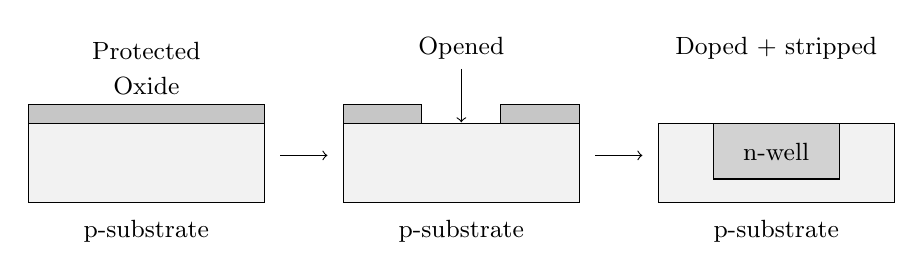
\begin{tikzpicture}[x=1cm,y=1cm,font=\small]
\foreach \shift/\lab in {0/Protected,4/Opened,8/{Doped + stripped}} {
\begin{scope}[xshift=\shift cm]
\draw[fill=gray!10] (0,0) rectangle (3,1);
\node[above] at (1.5,1.7) {\lab};
\node[below] at (1.5,-0.1) {p-substrate};
\end{scope}}
\draw[fill=gray!45] (0,1) rectangle (3,1.25);
\node[above] at (1.5,1.25) {Oxide};
\draw[fill=gray!45] (4,1) rectangle (5,1.25);
\draw[fill=gray!45] (6,1) rectangle (7,1.25);
\draw[->] (5.5,1.7)--(5.5,1.02);
\draw[fill=gray!35] (8.7,0.3) rectangle (10.3,1);
\node at (9.5,0.65) {n-well};
\draw[->] (3.2,0.6)--(3.8,0.6);
\draw[->] (7.2,0.6)--(7.8,0.6);
\end{tikzpicture}
\end{latin}
\caption{سه وضعیت انتخاب‌شده از ساخت چاه، بر پایه شکل \secnum{۱.۳۶} کتاب
\cite{weste}؛ همه مراحل \lr{Lithography} در این تصویر فشرده رسم نشده‌اند.
پهن‌تر بودن چاه از پنجره، اثر مفهومی انتشار جانبی است؛ اندازه‌ها واقعی نیستند.}
\label{fig:layout-well-stages}
\end{figure}

\lr{Diffusion} یعنی حرکت اتم‌های ناخالصی در ماده در شرایط مناسب حرارتی.
در \lr{Ion Implantation}، یون‌ها با میدان شتاب می‌گیرند و به سطح وارد می‌شوند.
کتاب هر دو را برای افزودن ناخالصی توضیح می‌دهد؛ نتیجه و پروفایل واقعی آن‌ها
به فرایند وابسته است. از نام ماسک \lr{Diffusion} نباید نتیجه گرفت تمام
ناحیه‌های موسوم به \lr{Diffusion} الزاماً با همان روش قدیمی ساخته شده‌اند.

\subsection{ساخت \lr{Gate} و معنای \lr{Self-aligned}}
پس از چاه، اکسید نازک \lr{Gate} و لایه \lr{Polysilicon} تشکیل می‌شوند.
در فرایند توضیحی کتاب، \lr{Chemical Vapor Deposition (CVD)} برای تشکیل
\lr{Poly} به کار می‌رود و ناخالصی مناسب رسانایی آن را افزایش می‌دهد.
با ماسک \lr{Poly}، فقط نوارهای موردنیاز باقی می‌مانند
\cite[شکل \secnum{۱.۳۷}]{weste}.

سپس انتخاب ناحیه‌های \(n^+\) برای \lr{nMOS} و تماس چاه انجام می‌شود.
\lr{Gate} موجود، ورود ناخالصی را در محل کانال مسدود می‌کند؛
بنابراین دو ناحیه \lr{Source} و \lr{Drain} در دو سوی همان \lr{Gate}
تشکیل می‌شوند. این \lr{Self-aligned Gate} به معنی خودترازی لبه‌های مرتبط با
\lr{Gate} است، نه بی‌نیازی کل تراشه از هم‌ترازی ماسک‌ها.

برای ناحیه‌های \(p^+\)، انتخاب نوع مخالف تکرار می‌شود تا \lr{Source/Drain}
ترانزیستور \lr{pMOS} و تماس بستر ساخته شوند.
ناحیه فعال \lr{nMOS} باید در بستر \lr{p} و ناحیه فعال \lr{pMOS} داخل چاه
\lr{n} قرار گیرد. فقط عوض کردن رنگ یا برچسب نقشه، این شرط فیزیکی را تامین نمی‌کند.

\subsection{عایق، \lr{Contact} و اتصال فلزی}
در مدل کتاب، عایق میان فلز و ناحیه‌های زیرین قرار می‌گیرد؛ ماسک \lr{Contact}
جاهایی را باز می‌کند که اتصال لازم است. سپس فلز نشانده و با ماسک خودش الگوگذاری می‌شود.
در مثال ساده، آلومینیوم و فرایند \lr{Sputtering} توصیف شده‌اند؛
این انتخاب مواد، مشخصه همان مدل توضیحی است، نه الزام همه فرایندها
\cite[شکل \secnum{۱.۳۸}]{weste}.

اگر چند لایه فلزی داشته باشیم، عایق، الگوگذاری فلز و اتصال‌های بین لایه‌ای
نیز لازم می‌شوند. شمار ماسک‌های واقعی و روش عایق‌سازی و متالیزاسیون می‌تواند
بسیار پیچیده‌تر باشد. در این بخش، هدف دنبال کردن نقش لایه‌هاست؛
نه ارائه دستور اجرایی آزمایشگاه ساخت.

\subsection{چرا مساحت مهم است؟}
بخش زیادی از مراحل روی ویفر و تعداد زیادی تراشه تکرار می‌شود؛
ازاین‌رو مساحت هر تراشه بر تعداد تراشه‌های قابل جاگذاری اثر دارد.
در یک برآورد هندسی، کاهش مساحت \(A\) در مساحت قابل‌استفاده ثابت ویفر
\(A_{\mathrm{wafer}}\)، تعداد خام را تقریباً به نسبت
\(A_{\mathrm{wafer}}/A\) افزایش می‌دهد.
این نسبت، برش لبه، خطوط جداسازی و \lr{Yield} را لحاظ نمی‌کند؛
پس هزینه دقیق تراشه فقط با شمار ترانزیستور یا این نسبت تعیین نمی‌شود.
این توضیح، برداشت ساده بخش \secnum{۱.۵.۲} کتاب از اهمیت مساحت را با فرض‌هایش روشن می‌کند.

\subsection{پرسش‌های ساخت با پاسخ}
\begin{enumerate}
\item \textbf{پس از پاک کردن ماسک اکسیدی، چرا چاه باقی می‌ماند؟}
چاه ناحیه‌ای با ناخالصی تغییرکرده داخل نیمه‌هادی است؛ اکسید پوشش انتخابی روی سطح بود.
\item \textbf{آیا \lr{Gate} با کانال تماس رسانشی مستقیم دارد؟}
در مدل ایدئال خیر؛ عایق نازک میان آن‌هاست. تقاطع در نمای بالا به معنی اتصال کوتاه نیست.
\item \textbf{چرا تماس بدنه \lr{pMOS} از نوع \(n^+\) است؟}
چون به بدنه \lr{n-well} وصل می‌شود؛ ناحیه‌های \(p^+\) آن ترانزیستور مربوط به \lr{Source/Drain} هستند.
\item \textbf{آیا شش ماسک معرفی‌شده تعداد ماسک‌های یک فناوری واقعی است؟}
خیر؛ این مجموعه برای توضیح مدار و مسیر ساخت فرض شده است و مراحل صنعتی بیشتری لازم است.
\end{enumerate}
